\vspace{1.0cm}
\section{Analysis of Uber's Effects on Taxi Market}
\subsection{Uber's Effects on Demand for Yellow Cabs}

\hspace{0.5cm} Uber grew dramatically since 2014 in NYC and the phenomenon caused the significant decrease in demand for yellow cabs. See Figure \ref{fig:Daily_trips} in Section 3. Moreover, Uber cut its fare at the end of January 2016 by approximately 15\% in NYC and it perhaps accelerated Uber's expansion. See 3.2.4. In this section, I estimate how Uber's growth and its fare cut affected demand for yellow cabs. I use data from February and March in 2015 and 2016 because the period in 2016 is a timing just after the fare cut and thus would be appropriate for estimation of the price elasticity at the time when Uber was rapidly expanding.\footnote{Furthermore, TLC changed the way of disclosure of locations in July 2016 so the data of the second half of the year would not be pertinent in this case.} I estimate the demand curve of yellow cabs with consideration of Uber's rise as follows.

\begin{equation}
\begin{split}
 log(Q^d_{ijh}) = \beta_0 + \beta_1 log(UberTrip_{ih}) + \beta_2 log(w_{ih}) + \gamma X_{ijh} +  \epsilon_{ijh} \label{eq:lnuber}
\end{split}
\end{equation}

\noindent This equation is similar to that in the previous section, but different in that 1) yellow cabs fare didn't change during the time period, so the variable is omitted, and 2) I add $log(UberTrip_{ih}$), the number of trips completed by Uber starting from location i. As TLC doesn't provide data on dropoff locations of trips by Uber, I just use information of pickup locations to calculate $log(UberTrip_{ih})$. From the pricing system Uber discloses, the theoretical fare of $\delta_{ij}$ without surge pricing can be calculated, but as it is highly correlated with $log(UberTrip_{ih})$, and the coefficient of the fare would overestimate cross price elasticity, I omit them for the sake of higher precision of regression. Hence, I consider the effect of the fare cut not directly, but indirectly using the regression result. Like wait time, the number of trips by Uber is also suspected endogenous because yellow cabs and Uber would be substitutes. Thus I instrument the variable with velocity outside Manhattan and also dummy variable of the year being 2016. $\mathbf{\bm{\gamma} X_{ijh}}$ are the same as before. I also change the number of medallions\footnote{Buchholz (2016) also analyzes the effect of boro taxis by adding 1,000 yellow cabs into inner Manhattan.} from 8,000 to 9,000, considering that the number of boro taxis increased after its introduction and thus the situation outside yellow cab zones should have become more competitive, leading more yellow cabs to drive in Manhattan.\footnote{Restrictions on supply flexibility for minifleets and owner-operated medallions (see 3.1.1) were removed, so that yellow cab drivers might have responded to market conditions elastically and could lead to the violation of the assumption. As I have no data on labor supply, I keep assuming that the number of medallions is fixed and invariant to date as before.} I have checked again in Appendix C that this change doesn't affect the main results.


\begin{table}[h]
\caption{Elasticity of Demand w.r.t Uber's Trips and Wait Time}\label{tab:lnuber_regression}\\

{
\def\sym#1{\ifmmode^{#1}\else\(^{#1}\)\fi}
\begin{center}
\begin{tabular}{l*{2}{c}}
\hline\hline
            &\multicolumn{1}{c}{(1)}&\multicolumn{1}{c}{(2)}\\
             &\multicolumn{1}{c}{\textit{log (Waiting Passengers)}}&\multicolumn{1}{c}{\textit{log (Waiting Passengers)}}\\
\hline
${\widehat{log\, (Uber\,Trip)}}$  &      -0.168\sym{***}&      -0.166\sym{***}\\
            &    (0.0188)         &    (0.0187)         \\
[1em]
${\widehat{log\, (Wait\, Time)}}$&      -0.247\sym{***}&      -0.223\sym{**} \\
            &    (0.0724)         &    (0.0721)         \\
\hline
\(N\)       &       55,244         &       55,244         \\
\(R^{2}\)   &       0.242         &       0.252         \\
Public Transportation Effect &         No            &             Yes        \\
\hline\hline
\multicolumn{3}{l}{\footnotesize Standard errors in parentheses}\\
\multicolumn{3}{l}{\footnotesize \sym{*} \(p<0.05\), \sym{**} \(p<0.01\), \sym{***} \(p<0.001\)}\\
\end{tabular}
\end{center}
}


\end{table}



The regression result is in Table \ref{tab:lnuber_regression}. Both of the elasticities are significant and the inclusion of public transportation effect has few impact. The elasticity of demand for yellow cabs with respect to Uber trips being approximately 0.17, which roughly shows the number of trips by yellow cab decreases by 1 for every 6 trips by Uber, suggests that Uber (and perhaps other ride-hailing services) generates new demand for door-to-door transportation rather than depriving passengers of yellow cabs. The result is compatible with the data shown in Section 3 that the total demand for taxi-like transportation actually increased from approximately 500,000 to 700,000 between 2013 and 2016.


Regarding the wait time elasticity, it is still below 1, but is much greater compared to that in 2012/2013 when Uber was not so popular. See Table \ref{tab:lnfare_regression} in the previous section. This result still remains unchanged even if I don't increase the number of medallions by 1,000 in Manhattan.  This implies that as Uber has become considered by passengers as the substitute for yellow cabs, they might wait for yellow cabs less patiently than before.

\begin{table}[h]
\centering
\caption{Elasticity of Demand w.r.t Uber's Trips with Cross Terms}\label{tab:lnuber_cross_regression}
\vspace{0.2cm}
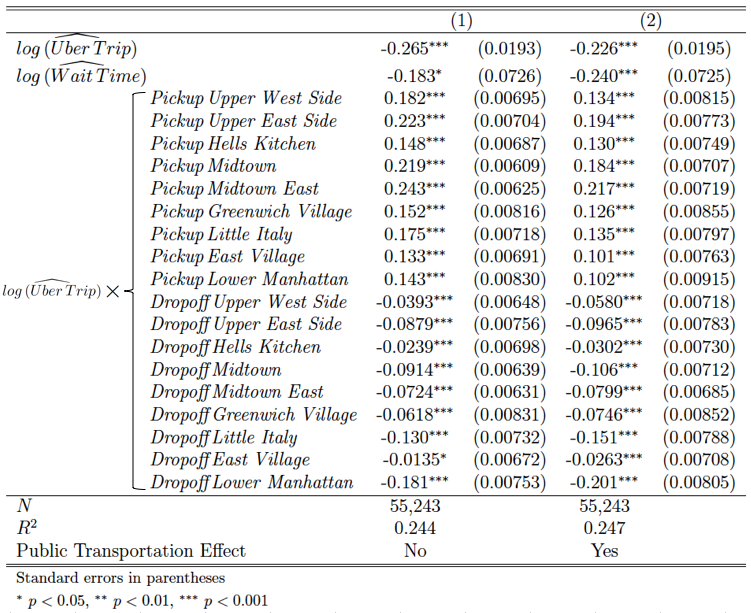
\includegraphics[width=16cm]{Tables/lnuber_cross_regression.png}
\end{table}


\indent As before, I also exercise regression replacing dummy variables of pickup and dropoff areas in $\mathbf{\bm{\gamma} X_{ijh}}$ above with the cross terms of "$log (Uber Trip)$ $\times$ pickup/dropoff areas" to check whether the elasticity of demand for yellow cabs with respect to Uber Trips are dependent on distance, as whether Uber actually cut its fare depends on it due to the application of minimum fare. Table \ref{tab:lnuber_cross_regression} shows the result and Figure \ref{fig:elasticity_lnuber} depicts the relationship between the distance of trips and the elasticities using the regression result with public transportation effects in Table \ref{tab:lnuber_cross_regression}. There are two important thresholds of distance. One is whether the minimum fare (\$7) is applied to Uber trips and the second is whether Uber is cheaper than yellow cabs. See also 3.2.4. The figure indicates that there is almost no relationship between distance and the elasticity of demand with respect to Uber Trips. This result indirectly suggests that Uber's fare cut\footnote{I assume here that the fare is just determined by the disclosed fare system and no surge pricing is exercised. According to Cohen et al. (2016), fare surged for less than 20\% of trips during the 5 hours from Monday to Thursday on average.} itself didn't decrease demand for yellow cabs, though it might have increased demand for Uber itself. In fact, Uber was already cheaper than yellow cabs even before fare cut conditional on minimum fare not being applied and hence there were few passengers who began to use Uber instead of yellow cabs just because the fare decreased. Furthermore, this supports the conclusion above that Uber mainly generated new demand rather than taking them from yellow cabs. 

\begin{figure}[h]
\centering
\caption{Estimate of Uber's Effect}\label{fig:elasticity_lnuber}
\vspace{0.2cm}
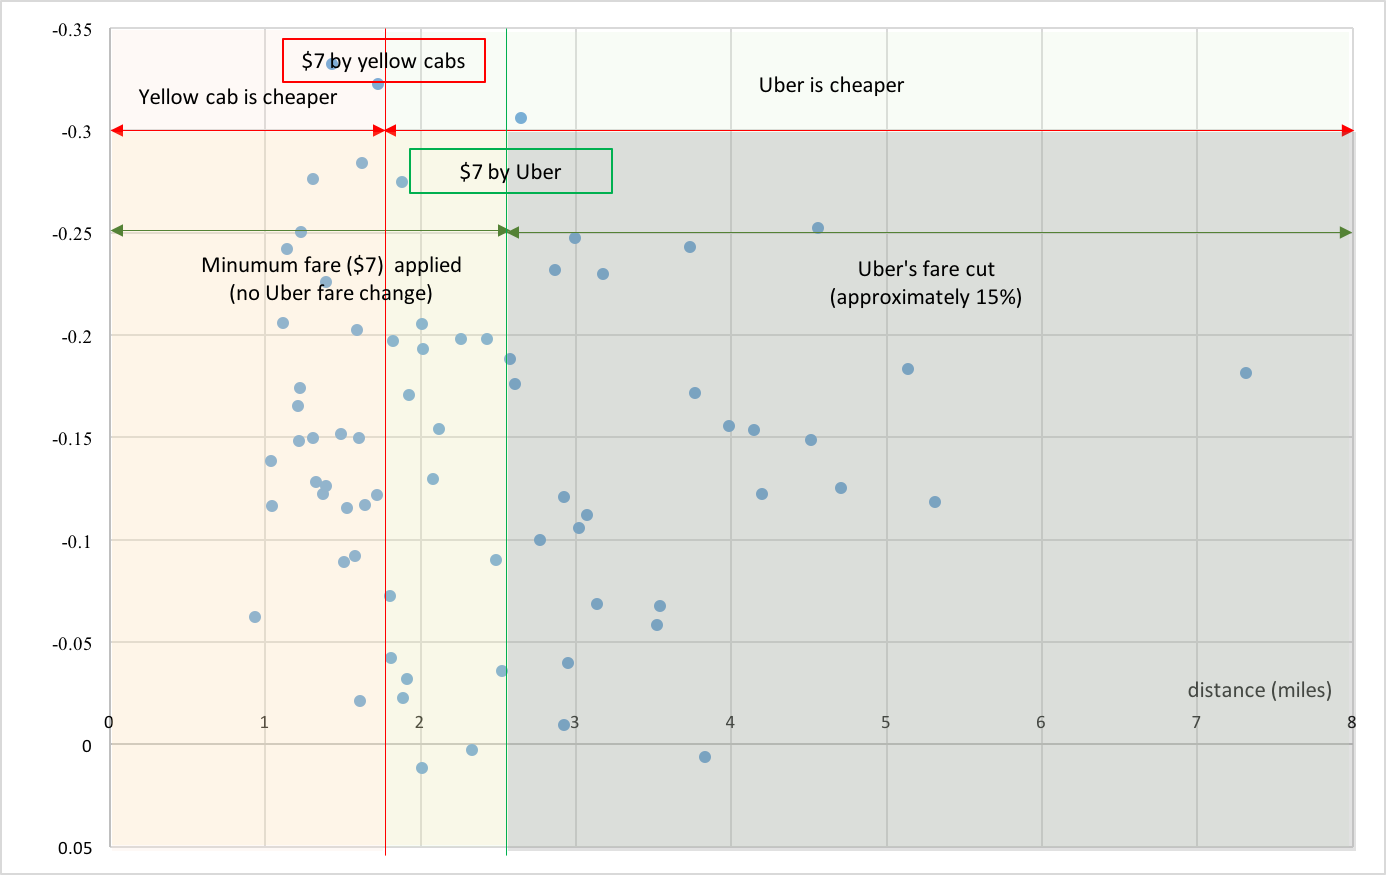
\includegraphics[width=16.5cm]{Figures/elasticity_lnuber.png}
\end{figure}


\vspace{0.5cm}

\subsection{Welfare Analysis of Uber's Rise}
\hspace{0.5cm} I measure consumer surpluses of yellow cabs and Uber as in 4.3, but as there was no price change after 2015 and no data regarding Uber's dropoff locations, I instead use wait time rather than price to calculate the consumer surpluses.\footnote{It's still possible that I use price elasticity estimated in the previous section to measure the consumer surplus, but it is likely that they have changed due to the rise of ride-hailing services.} I first exercise a regression with cross terms to estimate the pickup-location dependent elasticity of demand with respect to wait time and estimate the elasticity for each pickup area as in Table \ref{tab:each_lnuber}\footnote{The regression result and the variance-covariance matrix of the variables with public transportation effect to derive the elasticity for each pickup area are in Table \ref{tab:lnwaittime_uber_cross} and Table \ref{tab:vce_lnuber} in Appendix D.}. The method of calculation of consumer surplus is the same as shown in 4.3, but as I don't have sufficient data on Uber's trips, I assume that wait time, as well as the elasticities of demand with respect to the wait time for yellow cabs and Uber are identical and also that all trips by Uber starting in Manhattan end within Manhattan. Daily consumer surpluses during the peak time of both yellow cabs and Uber for each year are summarized in Table \ref{tab:welfare_waittime}. The consumer surplus of yellow cabs declined by 13 \% while that of Uber more than tripled, resulting in the total consumer surplus in 2016 being much higher than that in 2015.\footnote{As driver's labor supply is fixed in this model, producer surplus using search time cannot be calculated.} This shows that Uber generated new consumer surplus and is an evidence that ride-hailing services contribute to the higher social welfare.\footnote{Note again that as these consumer surpluses are lower bound, I impose some assumptions and I don't consider producer surplus and externalities like congestion, the result is just suggestive.}



\begin{table}[h]
\caption{Elasticity of Demand w.r.t Wait Time for Each Pickup Area}\label{tab:each_lnuber}
{
\def\sym#1{\ifmmode^{#1}\else\(^{#1}\)\fi}
\begin{center}
\scalebox{1}[1]{
\begin{tabular}{l*{11}{c}}
\hline\hline
                        
            & &\multicolumn{1}{c}{Elasticity}&
            
            \\

\hline
&\multicolumn{1}{l}{Central Park}      &   -0.502\sym{*} &
 (0.248)\\
&\multicolumn{1}{l}{Upper West Side} &   -0.443\sym{**} &
 (0.137)\\
&\multicolumn{1}{l}{Upper East Side} &  -0.140&	
 (0.168)\\
&\multicolumn{1}{l}{Hell's Kitchen} &  -0.652\sym{***}&
 (0.143)\\
\multicolumn{1}{l}{Pickup Area} & \multicolumn{1}{l}{Midtown} &  -0.802\sym{***}& (0.110)\\
&\multicolumn{1}{l}{Midtown East} &  -0.220&	(0.130)\\
&\multicolumn{1}{l}{Greenwich Village} &  -1.021\sym{***} &(0.205)\\
&\multicolumn{1}{l}{Little Italy} & -0.921\sym{***}&	(0.153)\\
&\multicolumn{1}{l}{East Village} &  -0.545\sym{***}& (0.146)\\
&\multicolumn{1}{l}{Lower Manhattan} &  -0.908\sym{***}& (0.156)\\

\hline\hline
\multicolumn{3}{l}{\footnotesize Standard errors in parentheses}\\
\multicolumn{3}{l}{\footnotesize \sym{*} \(p<0.05\), \sym{**}
 \(p<0.01\), \sym{***} \(p<0.001\)}\\
\end{tabular}
}
\end{center}
}

\end{table}












\begin{table}[h]
\caption{Daily Consumer Surplus by Yellow Cabs and Uber}\label{tab:welfare_waittime}\\

{
\def\sym#1{\ifmmode^{#1}\else\(^{#1}\)\fi}
\begin{center}
\begin{tabular}{l*{5}{c}}
\hline\hline
Year & Yellow Cabs (min.) & Uber (min.) & Total (min.)\\
\hline
 2015 & 7.82 M & 3.51 M & 11.33 M\\
 2016 & 6.86 M & 11.96 M & 18.82 M\\

 
 


\hline\hline
\end{tabular}
\end{center}
}


\end{table}

